\documentclass[border=10pt]{standalone}
% Shared visual language for CAML diagrams (pdflatex + Fira Sans/Mono).
% Native SVG output: build with latex (DVI) + dvisvgm, see build.sh. The
% PDF route (pdflatex + dvisvgm --pdf) turns every transparency into solid
% black/white blocks.
\def\pgfsysdriver{pgfsys-dvisvgm.def}
\usepackage[T1]{fontenc}
\usepackage[sfdefault]{FiraSans}
\usepackage[scale=0.92]{FiraMono}
\usepackage{amssymb}
\usepackage{tikz}
\usetikzlibrary{arrows.meta, positioning, shadows, fit, backgrounds, calc}

% --- palette ------------------------------------------------------------
\definecolor{ink}{HTML}{16202C}
\definecolor{muted}{HTML}{5B6B7F}
\definecolor{edge}{HTML}{47576B}
\definecolor{card}{HTML}{F7F9FC}
\definecolor{page}{HTML}{FFFFFF}

\definecolor{indigo}{HTML}{4B54C6}   \definecolor{indigobg}{HTML}{EDEEFC}
\definecolor{amber}{HTML}{C9740A}    \definecolor{amberbg}{HTML}{FCF0DE}
\definecolor{green}{HTML}{0E9E6B}    \definecolor{greenbg}{HTML}{E4F6EE}
\definecolor{purple}{HTML}{7A3CE0}   \definecolor{purplebg}{HTML}{F1E9FD}
\definecolor{rose}{HTML}{D23F72}     \definecolor{rosebg}{HTML}{FBE7EE}
\definecolor{slate}{HTML}{47576B}    \definecolor{slatebg}{HTML}{EDF1F6}

% --- node + arrow styles ------------------------------------------------
% A flat offset drop shadow: shadows.blur's faded shadows render as solid
% black boxes under the dvisvgm driver.
\tikzset{soft shadow/.style={drop shadow={shadow xshift=0pt, shadow yshift=-1.8pt,
                                          opacity=0.12, fill=ink}}}
\tikzset{
  base/.style={
    rounded corners=5pt, draw, line width=1pt, inner sep=8pt,
    font=\small, text=ink, align=center,
    soft shadow},
  card/.style   ={base, fill=card,     draw=muted!70},
  indigo/.style ={base, fill=indigobg, draw=indigo, text=ink},
  amber/.style  ={base, fill=amberbg,  draw=amber,  text=ink},
  green/.style  ={base, fill=greenbg,  draw=green,  text=ink},
  purple/.style ={base, fill=purplebg, draw=purple, text=ink},
  rose/.style   ={base, fill=rosebg,   draw=rose,   text=ink},
  slate/.style  ={base, fill=slatebg,  draw=slate,  text=ink},
  sub/.style={font=\scriptsize, text=muted},
  arrow/.style={-{Stealth[length=2.8mm,width=2.4mm]}, line width=1.1pt, draw=edge},
  arrowd/.style={-{Stealth[length=2.8mm,width=2.4mm]}, line width=1.1pt, draw=edge, dashed},
  alabel/.style={font=\scriptsize, text=muted, align=center, fill=page, inner sep=2pt},
  grouplbl/.style={font=\bfseries\footnotesize, text=ink},
}

% inline text helpers for two-tier node labels
\newcommand{\Hd}[1]{{\bfseries #1}}
\newcommand{\Sb}[1]{{\normalfont\scriptsize\textcolor{muted}{#1}}}
\newcommand{\Sbc}[2]{{\normalfont\scriptsize\textcolor{#1}{#2}}}

% White rounded card behind every diagram. The SVGs used to be transparent
% with dark ink, so labels drawn straight on the page vanished on GitHub's
% dark theme. It is drawn on its own lowest layer: the backgrounds
% library's `show background rectangle` would cover anything a diagram puts
% `on background layer` (pipeline.tex's sandbox box). banner.tex opts out
% with \camlcardfalse since it is its own dark card.
\newif\ifcamlcard \camlcardtrue
\pgfdeclarelayer{card}
\pgfsetlayers{card,background,main}
\tikzset{every picture/.append style={execute at end picture={%
  \ifcamlcard
    \begin{pgfonlayer}{card}
      \path[fill=page, draw=muted!22, line width=0.6pt, rounded corners=12pt]
        ([shift={(-12pt,-12pt)}]current bounding box.south west) rectangle
        ([shift={(12pt,12pt)}]current bounding box.north east);
    \end{pgfonlayer}
  \fi}}}

\begin{document}
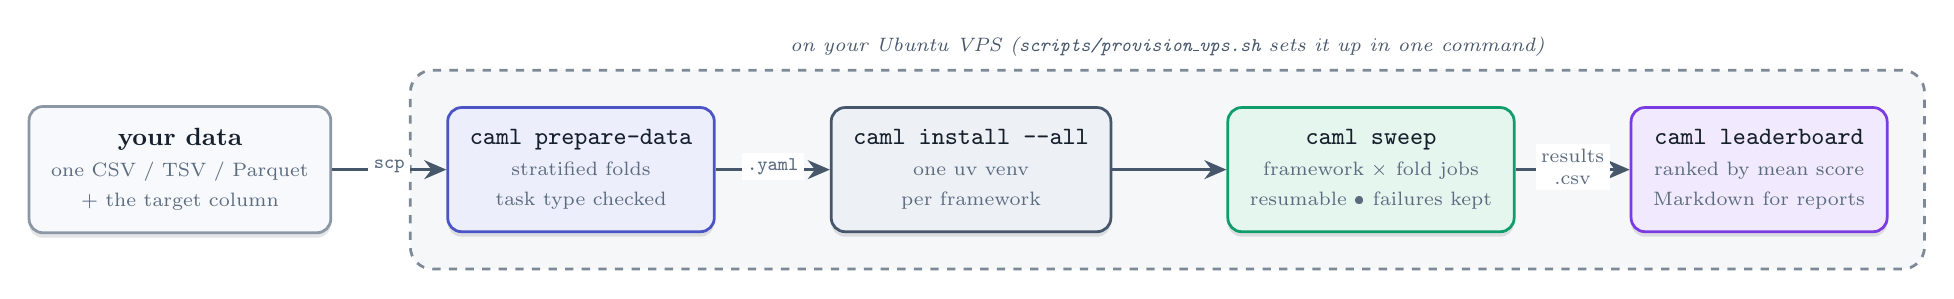
\begin{tikzpicture}[node distance=1.45cm]

  \node[card] (n0) {\Hd{your data}\\\Sb{one CSV / TSV / Parquet}\\\Sb{+ the target column}};
  \node[indigo, right=of n0] (n1) {\Hd{\texttt{caml prepare-data}}\\\Sb{stratified folds}\\\Sb{task type checked}};
  \node[slate, right=of n1] (n2) {\Hd{\texttt{caml install -{}-all}}\\\Sb{one uv venv}\\\Sb{per framework}};
  \node[green, right=of n2] (n3) {\Hd{\texttt{caml sweep}}\\\Sb{framework \texttimes\ fold jobs}\\\Sb{resumable \textbullet\ failures kept}};
  \node[purple, right=of n3] (n4) {\Hd{\texttt{caml leaderboard}}\\\Sb{ranked by mean score}\\\Sb{Markdown for reports}};

  % everything after the upload runs on the box (the YAML holds absolute paths)
  \begin{scope}[on background layer]
    \node[draw=slate!70, dashed, line width=1pt, rounded corners=8pt,
          fill=slate!5, fit=(n1)(n4), inner sep=13pt] (vps) {};
  \end{scope}
  \node[anchor=south, yshift=1pt] at (vps.north)
    {\Sbc{slate}{\itshape on your Ubuntu VPS (\texttt{scripts/provision\_vps.sh} sets it up in one command)}};

  \draw[arrow] (n0) -- (n1) node[alabel, midway, yshift=1pt] {\texttt{scp}};
  \draw[arrow] (n1) -- (n2) node[alabel, midway, yshift=1pt] {\texttt{.yaml}};
  \draw[arrow] (n2) -- (n3);
  \draw[arrow] (n3) -- (n4) node[alabel, midway, yshift=1pt] {results\\.csv};

\end{tikzpicture}
\end{document}
